\mySection{Experimental Results}

\subsection{Accuracy of Facial Recognition}
In our experiments, we select a variable n $\in$ $\{5, 10, 15, 20, 25, 30\}$ as our experimental parameter,
where n is the number of facial embeddings pre-computed per person. Simply put, n is the
number of photos collected from each individual before actually performing facial recognition.
Each time the experiment yields the number of faces recognized correctly, denoted by p.
We define another variable k to represent the number of faces in a testing set.
Finally, the correct rate $C_n$  for an experiment with respect to the parameter n can be evaluated by equation~\ref{eq:correct-rate}.

\begin{equation}
  \label{eq:correct-rate}
  C_n = p / k
\end{equation}

To assess how well our system can recognize faces with respect to different values of n,
we perform the experiment 6 times with varying values of n on each testing set. Moreover,
since we have three testing sets, we perform the experiment 18 times in total.
All values of $C_n$ collected from our experiments are presented in table~\ref{tab:exp-result-tab},
the visualization of which is shown in figure~\ref{fig:exp-result-chart}.
\vspace{0.5cm}

\begin{table}[!htb]
\centering
\caption{Correct rates for PyRollCall's facial recognition feature.} 
\begin{tabular}{@{}lcccccc@{}}
\toprule[2pt]
& \multicolumn{6}{c}{Number of embeddings pre-computed per person}                                                                                                                              \\ \addlinespace[0.5em]
                  & 5                          & 10                         & 15                         & 20                         & 25                         & 30                         \\ \midrule \addlinespace[0.5em]
Testing Set 1     & 8/20                       & 10/20                      & 15/20                      & 17/20                      & 17/20                      & 17/20                      \\
                  & \multicolumn{1}{c}{(40\%)} & \multicolumn{1}{c}{(50\%)} & \multicolumn{1}{c}{(75\%)} & \multicolumn{1}{c}{(85\%)} & \multicolumn{1}{c}{(85\%)} & \multicolumn{1}{c}{(85\%)} \\ \addlinespace[0.5em] \midrule \addlinespace[0.5em]
Testing Set 2     & 8/20                       & 10/20                      & 12/20                      & 13/20                      & 14/20                      & 14/20                      \\
                  & \multicolumn{1}{c}{(40\%)} & \multicolumn{1}{c}{(50\%)} & \multicolumn{1}{c}{(60\%)} & \multicolumn{1}{c}{(65\%)} & \multicolumn{1}{c}{(70\%)} & \multicolumn{1}{c}{(70\%)} \\ \addlinespace[0.5em] \midrule \addlinespace[0.5em]
Testing Set 3     & 9/20                       & 13/20                      & 14/20                      & 15/20                      & 15/20                      & 15/20                      \\
                  & \multicolumn{1}{c}{(45\%)} & \multicolumn{1}{c}{(65\%)} & \multicolumn{1}{c}{(70\%)} & \multicolumn{1}{c}{(75\%)} & \multicolumn{1}{c}{(75\%)} & \multicolumn{1}{c}{(75\%)} \\ \addlinespace[0.5em] \midrule[2pt] \addlinespace[0.5em]
Avg. Correct Rate & 41.67\%                    & 55\%                       & 68.33\%                    & 75\%                       & 76.67\%                    & 76.67\%                    \\ \addlinespace[0.5em]
\bottomrule[2pt]
\end{tabular}
\label{tab:exp-result-tab}
\end{table}

The results indicate that PyRollCall can achieve approximately \textbf{70\% to 85\%} of correct rate
for facial recognition at its best if \textbf{25 to 30} photos are collected in advance from each individual.
\vspace{0.5cm}

\begin{figure}[!htb]
  \centering
  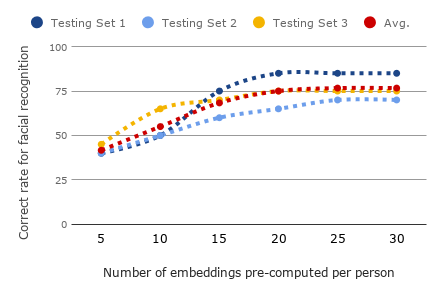
\includegraphics[width=0.8\linewidth]{figures/exp-result-chart.png}
  \caption{Visualization of the correct rates for PyRollCall's facial recognition feature.}
  \label{fig:exp-result-chart}
\end{figure}



\subsection{Analysis of Successful Facial Recognition}
In facial recognition, various factors such as face occlusion, face tilt, head rotation and aging
can pose a great challenge, and since our system is aimed to be practically used by educational
organization, we have taken these factors into consideration.
For instance, we have the legendary Hong Kong actor, Star Chow, as one of our participants. His photos
in the training set covers various facial expressions, hairstyles, angle of faces and even different age.
Figure~\ref{fig:correct-recog} demonstrates that even though most of his photos in the training set
are of the young Star Chow without wearing glasses, PyRollCall can still successfully recognize
the mid-aged Star Chow with glasses put on.

\begin{figure}[!htb]
  \centering
  \begin{subfigure}[b]{0.65\linewidth}
    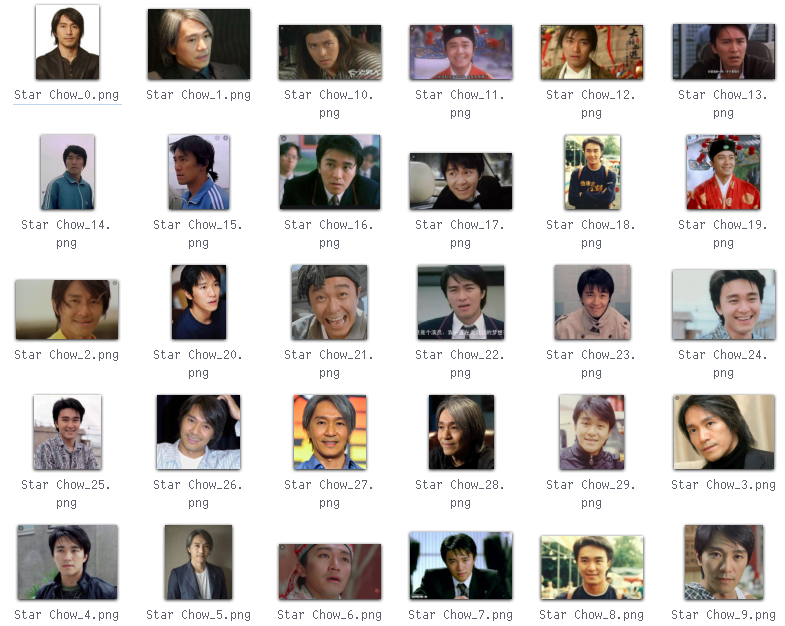
\includegraphics[width=\linewidth]{figures/star-chow-training-set.png}
    \caption{Star Chow's Training Set}
  \end{subfigure}
  \hfill
  \begin{subfigure}[b]{0.3\linewidth}
    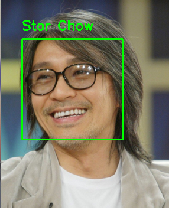
\includegraphics[width=\linewidth]{figures/star-chow-success.png}
    \caption{Star Chow}
  \end{subfigure}
  \caption{Example of successful facial recognition.}
  \label{fig:correct-recog}
\end{figure}
\vspace{0.5cm}



\subsection{Analysis of Faulty Facial Recognition}
In most cases, PyRollCall can recognize faces correctly as long as 25 to 30 photos are collected
beforehand from each individual. However, sometimes erroneous facial recognition can still take place,
especially when the targets wear makeup. Figure~\ref{fig:false-recog1} shows an example where
faulty facial recognition occurs due to makeup, rendering the essential structures of two faces
similar to each other.
\vspace{0.2cm}

\begin{figure}[!htb]
  \centering
  \begin{subfigure}[b]{0.3\linewidth}
    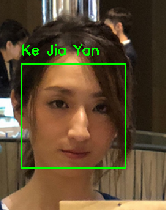
\includegraphics[width=\linewidth]{figures/false-recog-correct1.png}
    \caption{Ke Jia Yan}
  \end{subfigure}
  \begin{subfigure}[b]{0.3\linewidth}
    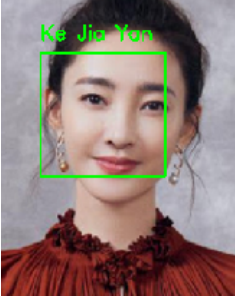
\includegraphics[width=\linewidth]{figures/false-recog-error1.png}
    \caption{Wang Li Kun}
  \end{subfigure}
  \caption{Erroneous facial recognition, example 1.}
  \label{fig:false-recog1}
\end{figure}

Another reason which can lead to error in facial recognition is insufficient amount of photos collected,
as shown in figure~\ref{fig:false-recog2}. Even with 30 photos collected for each individual in advance,
sometimes the result can still be faulty.% Collecting 30 photos from each individual is already pretty
%difficult, it would be impractical to require students to provide more than 30 photos.
\vspace{0.2cm}

\begin{figure}[!htb]
  \centering
  \begin{subfigure}[b]{0.3\linewidth}
    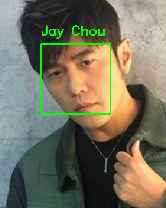
\includegraphics[width=\linewidth]{figures/false-recog-correct2.png}
    \caption{Jay Chou}
  \end{subfigure}
  \begin{subfigure}[b]{0.3\linewidth}
    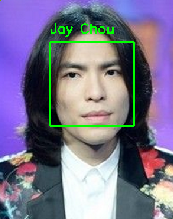
\includegraphics[width=\linewidth]{figures/false-recog-error2.png}
    \caption{Jam Hsiao}
  \end{subfigure}
  \caption{Erroneous facial recognition, example 2.}
  \label{fig:false-recog2}
\end{figure}
\vspace{0.2cm}



\subsection{Integration with Educational Organization}
Finally, in this section we discuss the effect of replacing traditional roll calls with PyRollCall.
Currently, our experimental results show that PyRollCall can recognize faces with an accuracy of 70\% to 85\%
at its best, provided that 25 to 30 photos are collected from each individual in advance.
It is unknown to us whether collecting more than 30 photos from each person can yield higher correct rate
for facial recognition, but 30 photos is already a great amount of photos to collect, even for
public figures whose photos can be easily acquired on the Internet. Furthermore, collecting, organizing and pre-computing
facial embeddings from photos will take quite a bit of time. In our experiments, the time we spent on pre-computing
facial embeddings is presented in table~\ref{tab:time-spent-on-training}.

\begin{table}[!htb]
\centering
\caption{Time spent on pre-computing facial embeddings for 20 people.} 
\begin{tabular}{@{}lcccccc@{}}
\toprule[2pt]
& \multicolumn{6}{c}{Number of embeddings pre-computed per person}                    \\ \addlinespace[0.5em]
                  & 5       & 10      & 15      & 20       & 25       & 30            \\ \midrule \addlinespace[0.5em]
Time spent (secs) & 340.6   & 625.3   & 943.5   & 1296.6   & 1731.8   & 1946.5        \\ \addlinespace[0.5em]
\bottomrule[2pt]
\end{tabular}
\label{tab:time-spent-on-training}
\end{table}

% TODO below
Next, we discuss the time that can be conserved if a teacher replaces the traditional roll calls
with PyRollCall.
With sufficient photos of students provided and their facial embeddings pre-computed,
the system will be able to detect and recognize faces correctly. Currently, as shown

to save time in classes, teachers and students will have to spend equivilently extra amount of time
before classes on the tasks such as collecting photos and pre-computing facial embeddings.
This proves that there is a trade off between convenience and efficiency.
\vspace{0.2cm}

